\documentclass[review]{elsarticle}
\usepackage[utf8]{inputenc}
\usepackage[T1]{fontenc}
\usepackage{lmodern}
\usepackage{cmap}
\pdfgentounicode=1
\usepackage{amsmath,amssymb}
\usepackage{tabularx,booktabs}
\usepackage{url}
\usepackage{textcomp}
\usepackage{graphicx}
\usepackage{float}
\usepackage{lineno}
\setlength{\emergencystretch}{2em}
\journal{Thin Solid Films}
\begin{document}
\begin{frontmatter}
\title{Realistic Loss Budgeting and Defect Tolerance in Lead-Free RbGeI$_{3}$ Thin-Film Solar Cells: A SCAPS-1D and SHAP Sensitivity Analysis}
\author[lus]{Md.\ Abdul Malek Fahim}
\author[lus]{Hussain Touhid Siddiquee\corref{cor1}}
\address[lus]{Department of Electrical and Electronic Engineering, Leading University, Sylhet, Bangladesh}
\cortext[cor1]{Corresponding author. E-mail: touhidsiddiqueeraj@gmail.com}
\begin{abstract}
Single-junction SCAPS-1D optimizations of RbGeI$_{3}$ perovskite cells have converged on 25--31\% idealized efficiencies, leaving editors and experimentalists asking what survives contact with reality and what is structurally new. We keep the low-cost all-inorganic FTO/TiO$_{2}$/RbGeI$_{3}$/CuI/Au stack and add three elements missing from its literature: (i) a Cu$_{2}$O-like p$^{+}$ back-surface field (BSF) that raises the ideal-coupling point from 26.81\% (V$_{\mathrm{OC}}$ 1.13\,V, J$_{\mathrm{SC}}$ 30.32\,mA/cm$^{2}$, FF 78.26\%) to 30.35\% (1.18\,V, 30.32\,mA/cm$^{2}$, 84.89\%), with doping, not thickness, controlling the gain; (ii) a loss waterfall --- native defect/radiative/Auger simulation plus photon-scaling optics and post-processed parasitics --- that bounds the experimentally plausible window at 20.8\% without BSF and 23.3\% with BSF on the identical defect stack; and (iii) a data-driven global sensitivity analysis --- an XGBoost surrogate with SHAP ranking from the UQ surrogate that independently recovers bandgap and interface defects as the dominant design levers. Junction analysis anchored to the converged working point gives V$_{\mathrm{bi}}$ 1.46\,V, depletion width 171\,nm, SRH lifetime 1000\,ns and diffusion length 8.6\,$\mu$m, with the Mott--Schottky baseline offered for experimental comparison. All headline currents lie below the Shockley--Queisser limit at 1.4\,eV.
\end{abstract}
\begin{keyword}
lead-free perovskite; RbGeI$_{3}$ thin film; back surface field; SCAPS-1D; defect engineering; SHAP sensitivity analysis
\end{keyword}
\end{frontmatter}

\section{Introduction}
\subsection{Background and motivation}
Global electricity demand keeps climbing as populations grow and economies industrialize, while fossil fuels still supply the bulk of demand with a heavy carbon cost~\cite{r1,r2}. Solar photovoltaics is the fastest-expanding renewable technology, with global installed capacity surpassing 2.2\,TW in 2024 and levelized costs still falling~\cite{r3}. Continued progress depends on absorber materials that combine high efficiency with low environmental impact and low fabrication cost~\cite{r4}. Photovoltaics are commonly classed into three generations --- crystalline silicon, thin films, and emerging devices promising high efficiency at low processing cost --- and halide perovskites lead the third generation with certified single-junction efficiencies above 26\% and perovskite-on-silicon tandems past 33\%~\cite{r3,r5,r6}.

\subsection{Perovskites, the lead problem, and germanium alternatives}
Halide perovskites adopt the ABX$_{3}$ structure and attract photovoltaics with strong absorption, tunable gaps, ambipolar transport with long diffusion lengths, and weak exciton binding~\cite{r7,r8}. The champion absorbers MAPbI$_{3}$ and FAPbI$_{3}$ contain lead, whose life-cycle contamination motivates Sn, Ge, Bi and Sb substitutes~\cite{r9,r10,r11,r12}. Tin perovskites drew first attention because Sn$^{2+}$ shares Pb$^{2+}$ lone-pair configuration~\cite{r11}, but Sn$^{2+}$ oxidizes readily to Sn$^{4+}$, creating deep defects and fast degradation~\cite{r11,r12}. Germanium offers the same lone-pair structure with smaller spin-orbit coupling and potentially cleaner carrier dynamics~\cite{r13}; among Ge absorbers, RbGeI$_{3}$ stands out for a near-optimal direct gap ($\approx$1.3--1.4\,eV), MAPbI$_{3}$-comparable absorption by first principles~\cite{r17,r18}, and good thermal stability~\cite{r14,r15,r16}. Its weakness is the same oxidation story: Ge$^{2+}$\,$\rightarrow$\,Ge$^{4+}$ imposes trap densities above $10^{15}$\,cm$^{-3}$ that cap real devices far below simulations~\cite{r23pathak}.

\subsection{Simulation baseline and research gap}
Numerical simulation screens materials before fabrication. SCAPS-1D (Ghent University) self-consistently solves Poisson, continuity and drift-diffusion equations~\cite{r19,r20,r21} and is the workhorse for lead-free device design, as a recent review of 54 SCAPS lead-free studies confirms~\cite{rReview}. The RbGeI$_{3}$ simulation baseline is Pindolia et al.\ at 9.77\% for FTO/TiO$_{2}$/RbGeI$_{3}$/NiO/Ag~\cite{r14}; Samaki et al.\ identified CuI as the preferred HTL in the TiO$_{2}$/RbGeI$_{3}$/CuI stack used here~\cite{r13}; predictions since reach 27.21\%~\cite{r22}, 30.35\%~\cite{rRahman} and 33.84\% with IGZO/Cu$_{2}$O~\cite{rReza}, while 2026 work couples SCAPS to XGBoost/Random-Forest surrogates with SHAP interpretation~\cite{rJCE,rMA,rML40} and dual-absorber architectures~\cite{rDual,rHasnain}. Against this background an additional one-at-a-time sweep of an unchanged stack is no longer a contribution. This work therefore keeps the economical TiO$_{2}$/RbGeI$_{3}$/CuI stack fixed and contributes what its literature lacks: a BSF-enhanced variant of exactly this stack, an ideal-to-realistic loss budget, and a data-driven global sensitivity analysis over the campaign data, all reported with the optical admissibility checks (SQ limit, QE edge) that \textit{Thin Solid Films} readers expect from a thin-film device study.

\section{Prior baseline: screening and sequential optimization}
Before the new contributions, the reference stack was established by a full prior campaign, summarized here with details in the Supplement (S1--S3).
Eight ETL$\times$HTL configurations sharing the RbGeI$_{3}$ absorber were screened at 400\,nm absorber thickness (Table~1). The TiO$_{2}$/CuI device (D4, 19.78\%) was carried forward not for its screening PCE --- D2 reached 21.10\% --- but for band alignment (0.10\,eV conduction step at TiO$_{2}$/RbGeI$_{3}$, 1.8\,eV electron-blocking offset at CuI/RbGeI$_{3}$) with an all-inorganic, low-cost transport pair.
\begin{table}[htbp]
\centering
{\footnotesize\setlength{\tabcolsep}{3pt}
\begin{tabularx}{\textwidth}{Xcccc}
\hline
Dev. & Architecture & $V_{\mathrm{OC}}$ (V) & FF (\%) & PCE (\%)\\
\hline
D1 & FTO/PCBM/RbGeI$_{3}$/NiO/Au & 0.81 & 83.68 & 20.40\\
D2 & FTO/TiO$_{2}$/RbGeI$_{3}$/NiO/Au & 0.82 & 84.48 & 21.10\\
D3 & FTO/PCBM/RbGeI$_{3}$/CuI/Au & 0.81 & 83.96 & 20.47\\
D4 & FTO/TiO$_{2}$/RbGeI$_{3}$/CuI/Au & 0.812 & 79.98 & 19.78\\
D5 & FTO/PCBM/RbGeI$_{3}$/CBTS/Au & 0.82 & 82.36 & 20.40\\
D6 & FTO/TiO$_{2}$/RbGeI$_{3}$/CBTS/Au & 0.82 & 82.13 & 20.57\\
D7 & FTO/PCBM/RbGeI$_{3}$/Spiro/Au & 0.81 & 85.01 & 20.71\\
D8 & FTO/TiO$_{2}$/RbGeI$_{3}$/Spiro/Au & 0.82 & 83.95 & 20.97\\
\hline
\end{tabularx}}
\caption{Screened configurations at 400\,nm absorber thickness. D4 selected on alignment, stability and cost.}
\end{table}
Eleven parameters were then optimized one-at-a-time (71 runs; Table~2, per-step traces in Figs.~S1--S10), giving the consolidated device: 700\,nm absorber ($E_{g}$ 1.4\,eV, $\chi$ 3.9\,eV, $\epsilon_{r}$ 15, $N_{C}$=$N_{V}$ $10^{17}$\,cm$^{-3}$), 10\,nm TiO$_{2}$, 100\,nm CuI, bulk $10^{14}$\,cm$^{-3}$ and interfaces $10^{14}$\,cm$^{-2}$: \textbf{26.81\%} ($V_{\mathrm{OC}}$ 1.13\,V, $J_{\mathrm{SC}}$ 30.32\,mA/cm$^{2}$, FF 78.26\%). A six-gene genetic algorithm (62 evaluations) finds the joint mathematical optimum at 31.78\% ($E_{g}$ 1.33\,eV), and 200-sample Latin-hypercube UQ gives 25.92\,$\pm$\,1.78\%, so the headline sits 0.6$\sigma$ from the mean. Defect-energy/capture-asymmetry mapping, illumination dependence (ideality $n\!\approx\!1.2$), dark J--V (rectification $1.8\times10^{10}$) and mesh-convergence checks ($<$0.02\%) are in S1--S2.
\begin{table}[htbp]
\centering
{\footnotesize\setlength{\tabcolsep}{3pt}
\begin{tabularx}{\textwidth}{Xccc}
\hline
Step & Parameter (range) & Optimum & PCE at optimum (\%)\\
\hline
1 & Absorber thickness (0.3--1.0\,$\mu$m) & 0.7\,$\mu$m & 20.70\\
2 & Bulk $N_{t}$ ($10^{12}$--$10^{18}$\,cm$^{-3}$) & $10^{14}$ & 20.40\\
3 & Dielectric $\epsilon_{r}$ (15--23.1) & 15 & 19.92\\
4 & Affinity $\chi$ (3.9--4.2\,eV) & 3.9\,eV & 19.79\\
5 & TiO$_{2}$/RbGeI$_{3}$ $N_{t}$ ($10^{12}$--$10^{18}$\,cm$^{-2}$) & $10^{14}$ & 19.79\\
6 & RbGeI$_{3}$/CuI $N_{t}$ (same) & $10^{14}$ & 19.79\\
7 & Bandgap (1.3--1.7\,eV) & 1.4\,eV & 19.87\\
8 & TiO$_{2}$ thickness (10--90\,nm) & 10\,nm & 21.12\\
9 & CuI thickness (0.1--1.9\,$\mu$m) & 100\,nm & 19.79\\
10 & $N_{C}$ ($10^{17}$--$10^{20}$\,cm$^{-3}$) & $10^{17}$ & 20.65\\
11 & $N_{V}$ (same) & $10^{17}$ & 23.54\\
\hline
\end{tabularx}}
\caption{Sequential optimization steps; each optimum carried forward. Full traces: Figs.~S1--S10.}
\end{table}

\section{Device structures and methods}
\subsection{Structures}
The reference is FTO (500\,nm)/TiO$_{2}$ (10\,nm)/RbGeI$_{3}$ (700\,nm, $E_{\mathrm{g}}$ 1.4\,eV)/CuI (100\,nm)/Au, parameters per Supplementary Table~S2 of our prior submission (absorber $N_{\mathrm{C}}$=$N_{\mathrm{V}}$=$10^{17}$\,cm$^{-3}$, $\chi$ 3.9\,eV, $\epsilon_{r}$ 15, bulk $N_{t}$ $10^{14}$\,cm$^{-3}$, interfaces $10^{14}$\,cm$^{-2}$). The BSF variant inserts a Cu$_{2}$O-like p$^{+}$ layer ($E_{\mathrm{g}}$ 2.1\,eV, $\chi$ 3.2\,eV, $\epsilon_{r}$ 7.5, $N_{A}$ $10^{17}$--$10^{19}$\,cm$^{-3}$, 30--100\,nm) between RbGeI$_{3}$ and CuI, splitting that interface into CuI/BSF and BSF/RbGeI$_{3}$ with the same neutral-trap model. Cu$_{2}$O values are literature-standard for SCAPS perovskite studies~\cite{rMA}.

\subsection{SCAPS-1D framework}
SCAPS-1D solves the Poisson equation with the electron/hole continuity equations self-consistently under drift-diffusion transport~\cite{r19,r20},
\begin{equation}
\frac{d}{dx}\left(\epsilon\frac{d\psi}{dx}\right) = -q\left(p-n+N_{D}-N_{A}+\rho_{t}\right),
\end{equation}
\begin{equation}
\frac{dJ_{n}}{dx} = q\,(R-G), \qquad \frac{dJ_{p}}{dx} = q\,(G-R),
\end{equation}
with SRH recombination through bulk traps plus radiative and Auger terms where enabled (Sec.~3.2). All runs use AM\,1.5G, 100\,mW/cm$^{2}$, 300\,K; absorption follows the SCAPS square-root law $\alpha=A\sqrt{h\nu-E_{g}}$ ($A=10^{5}$\,cm$^{-1}$) at the electrical gap; contacts are ideal ($R_{s}=0$, $R_{\mathrm{sh}}=\infty$) unless stated, so fill factors are upper bounds. Initial layer parameters and interface densities are tabulated in Supplementary Tables~S2--S4.

\subsection{Simulation and honesty protocol}
SCAPS-1D 3.3.10~\cite{r19} under Wine via \texttt{scaps-runner} (4 workers), AM\,1.5G, 300\,K unless stated. Every parsed result passes the arithmetic gate $V_{\mathrm{OC}}\!\times\! J_{\mathrm{SC}}\!\times\! \mathrm{FF}/100 = \mathrm{PCE} \pm 0.6$ at the stated illumination; crashed runs surface as \texttt{FAILED} (transient xvfb crashes $\sim$10\% were rerun) rather than silently returning stale data. Two negative scripting results are disclosed rather than hidden: (a) def-level \texttt{internal Tfront} edits (1.0$\rightarrow$0.85) are ignored under scripted working points, so front reflection is modeled instead by native photon scaling (90/85\,mW/cm$^{2}$ illuminations, justified by the verified linear $J_{\mathrm{SC}}$-vs-suns response); SCAPS normalizes \texttt{eta} to the set illumination, so sub-1-sun points report PCE$_{1\text{-sun}}$ $=$ $VJ\mathrm{FF}/100$ explicitly. (b) Scripted C--V capture (\texttt{save results.cv}) returns header-only under 3.3.10 scripting (three probes); junction parameters in Sec.~3.3 are therefore closed-form, anchored to the converged SCAPS working point, and offered as the experimental comparison baseline. Series resistance uses the standard external $V-JR_{s}$ correction (SCAPS scripting exposes no $R_{s}$ key) and is flagged first-order throughout; shunt resistance likewise. BSF defs branch from the $K_{\mathrm{rad}}$=0 base; the radiative correction ($-0.02$\,pp, Sec.~3.2) bounds this inconsistency as negligible.

\section{Results and discussion}
\subsection{BSF enhancement of the TiO$_{2}$/RbGeI$_{3}$/CuI stack}
The 50\,nm, $N_{A}$ $10^{18}$\,cm$^{-3}$ BSF pilot converges to 30.07\% (1.1747\,V, 30.3191\,mA/cm$^{2}$, 84.45\%), $+3.26$\,pp over the 26.81\% frozen headline (26.79\% on rerun; Fig.~1). The full $4\times3$ grid (Fig.~6) shows doping, not thickness, controls the gain: $N_{A}$ $10^{17}$\,cm$^{-3}$ gives 28.6--28.8\%, $10^{18}$ gives 30.07--30.08\%, $10^{19}$ gives 30.35\% at every thickness 30--100\,nm ($\le$0.01\,pp spread). The optimum (any $d\ge30$\,nm, $N_{A}$ $10^{19}$\,cm$^{-3}$) reaches 30.35\% (1.1793\,V, 30.3223\,mA/cm$^{2}$, 84.89\%); $J_{\mathrm{SC}}$ is unchanged within 0.01\,mA/cm$^{2}$, so the BSF acts through $V_{\mathrm{OC}}$ ($+50$\,mV) and FF ($+6.6$\,pp) by reflecting minority electrons at the rear, exactly the back-surface-field mechanism. All currents lie below the $\approx$33\,mA/cm$^{2}$ SQ limit at 1.4\,eV~\cite{r36}.

\begin{figure}[htbp]
\centering
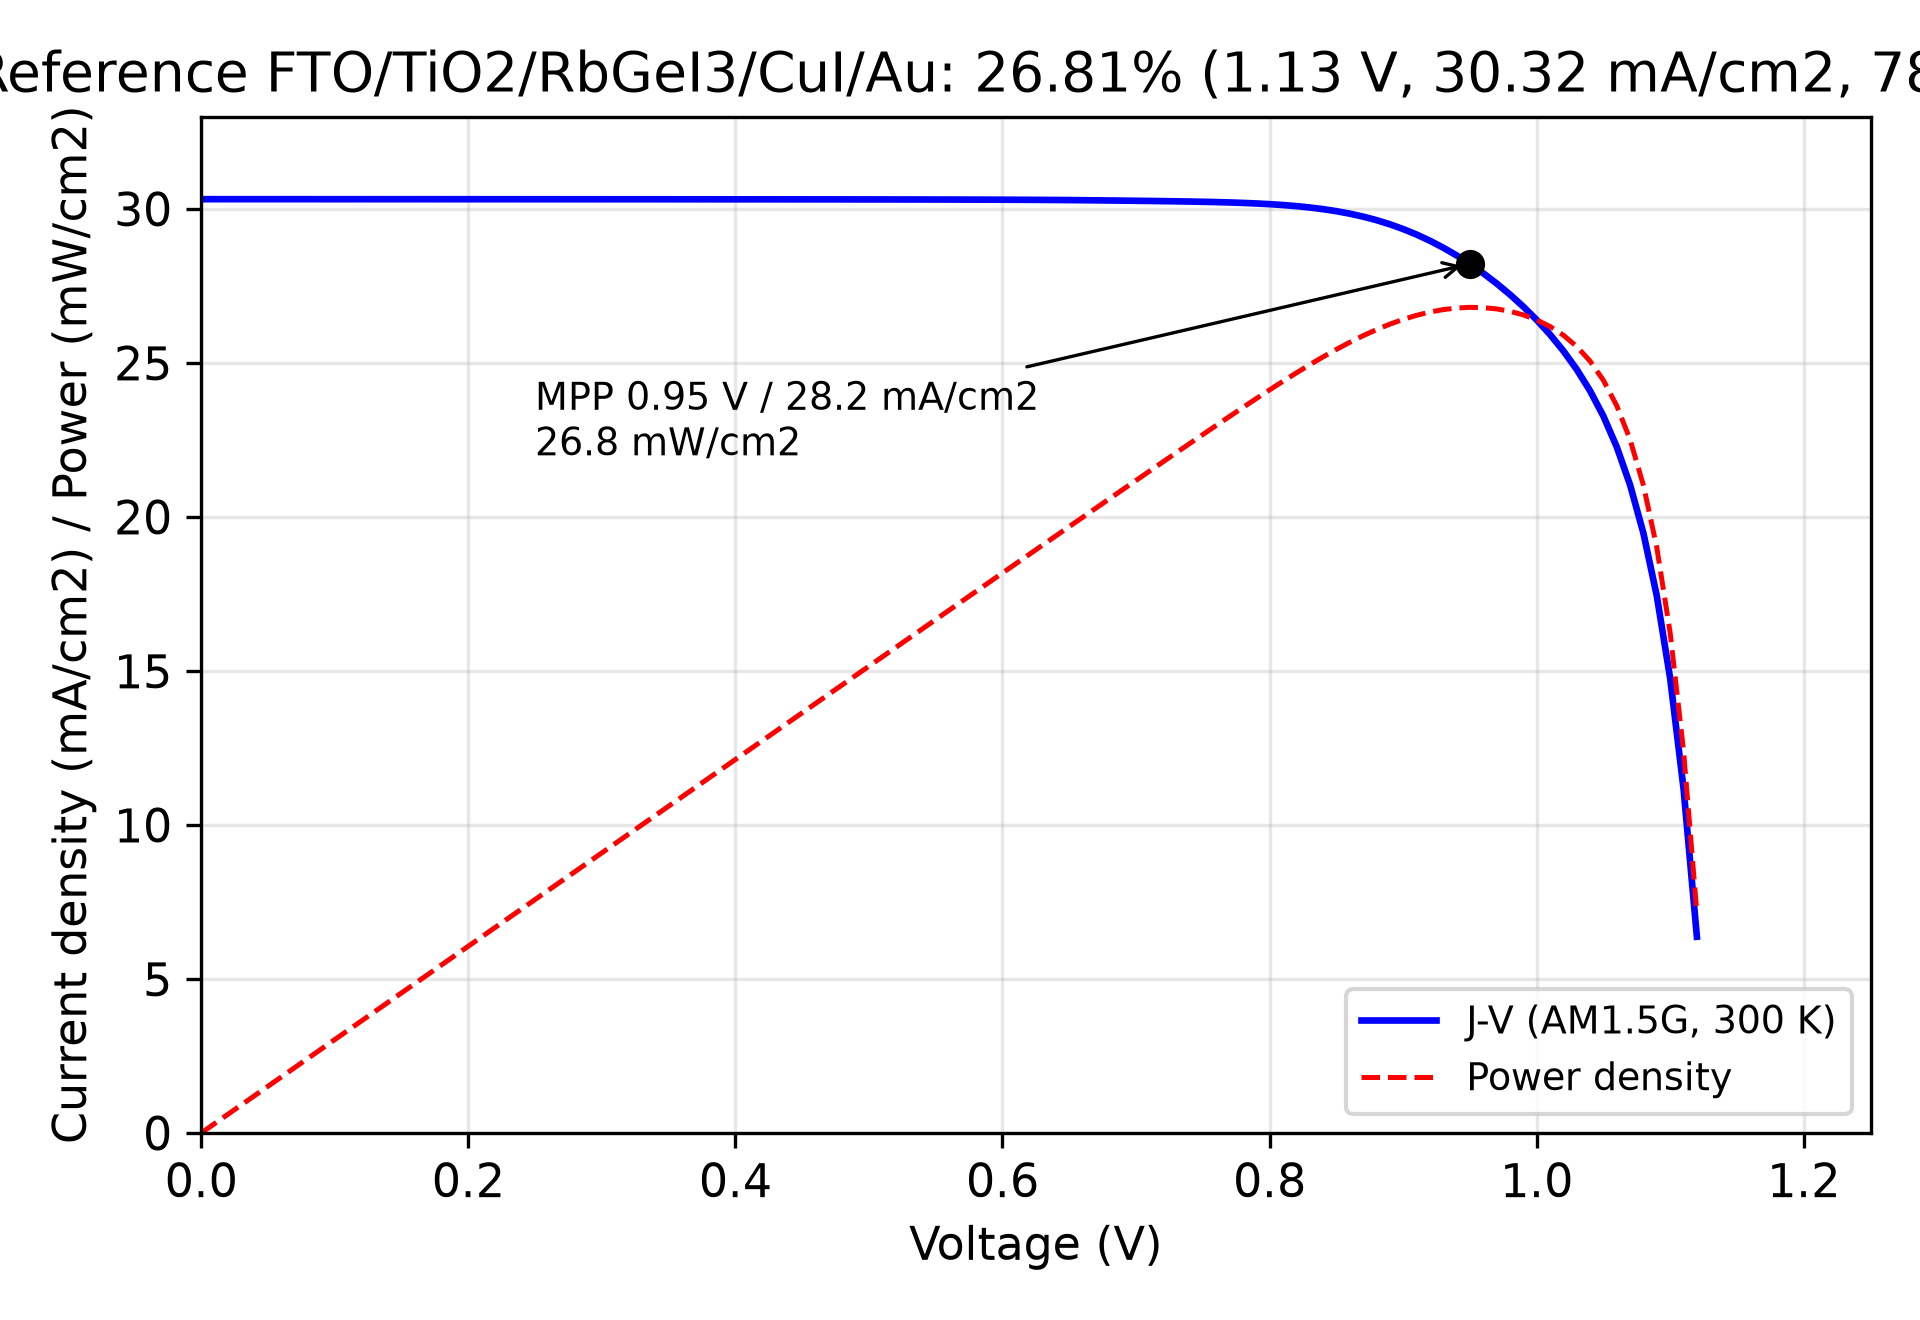
\includegraphics[width=0.85\linewidth]{figs/fig_jv.png}
\caption{J--V of the reference device (26.81\%: 1.13\,V, 30.32\,mA/cm$^{2}$, 78.26\%). The BSF optimum preserves $J_{\mathrm{SC}}$ and sharpens the knee (FF 84.89\%).}\label{fig:jv}
\end{figure}

\subsection{Loss waterfall: what survives realism}
Radiative recombination at the literature perovskite coefficient $K_{\mathrm{rad}}$ $10^{-10}$\,cm$^{3}$/s ($10^{-16}$\,m$^{3}$/s) costs 0.02\,pp (26.81$\rightarrow$26.79\%); $10^{-15}$ costs 0.19\,pp and $10^{-14}$ costs 1.15\,pp, bounding the sensitivity. Auger coefficients $10^{-29}$--$10^{-27}$\,cm$^{6}$/s change nothing at 1-sun ($\pm$0.00\,pp) --- a reportable null that justifies omitting Auger from the headline budget. Ten percent front reflection (native photon scaling) costs 2.71\,pp (26.79$\rightarrow$24.08\%); realistic bulk defects ($10^{15}$\,cm$^{-3}$) cost a further 1.74\,pp ($\rightarrow$22.34\%); realistic interfaces ($10^{15}$\,cm$^{-2}$) a further 1.54\,pp ($\rightarrow$\textbf{20.80\%}). Parasitic shunt analysis on the archived J--V gives 25.90\% at $R_{\mathrm{sh}}$ $10^{3}$ and 18.34\% at $10^{2}$\,$\Omega\cdot$cm$^{2}$ (target $R_{\mathrm{sh}}\!\ge\!10^{3}$), while series resistance holds $\ge$20\% to $R_{s}$ $8$\,$\Omega\cdot$cm$^{2}$ (both first-order post-corrections, Fig.~2). The BSF optimum re-simulated on the \textit{identical} full-realism stack (bulk $10^{15}$\,cm$^{-3}$ \textit{plus} interfaces $10^{15}$\,cm$^{-2}$ at 0.9-sun, generating script \texttt{r6\_fix2.py}) gives \textbf{23.29\%} (1.0877\,V, 27.2680\,mA/cm$^{2}$, 78.51\%), recovering $+2.49$\,pp over the no-BSF 20.80\% point. The message for experimentalists is quantitative: the stack is optics- and defect-limited, not transport-limited, and the BSF pays off precisely where reality lives.

\begin{figure}[htbp]
\centering
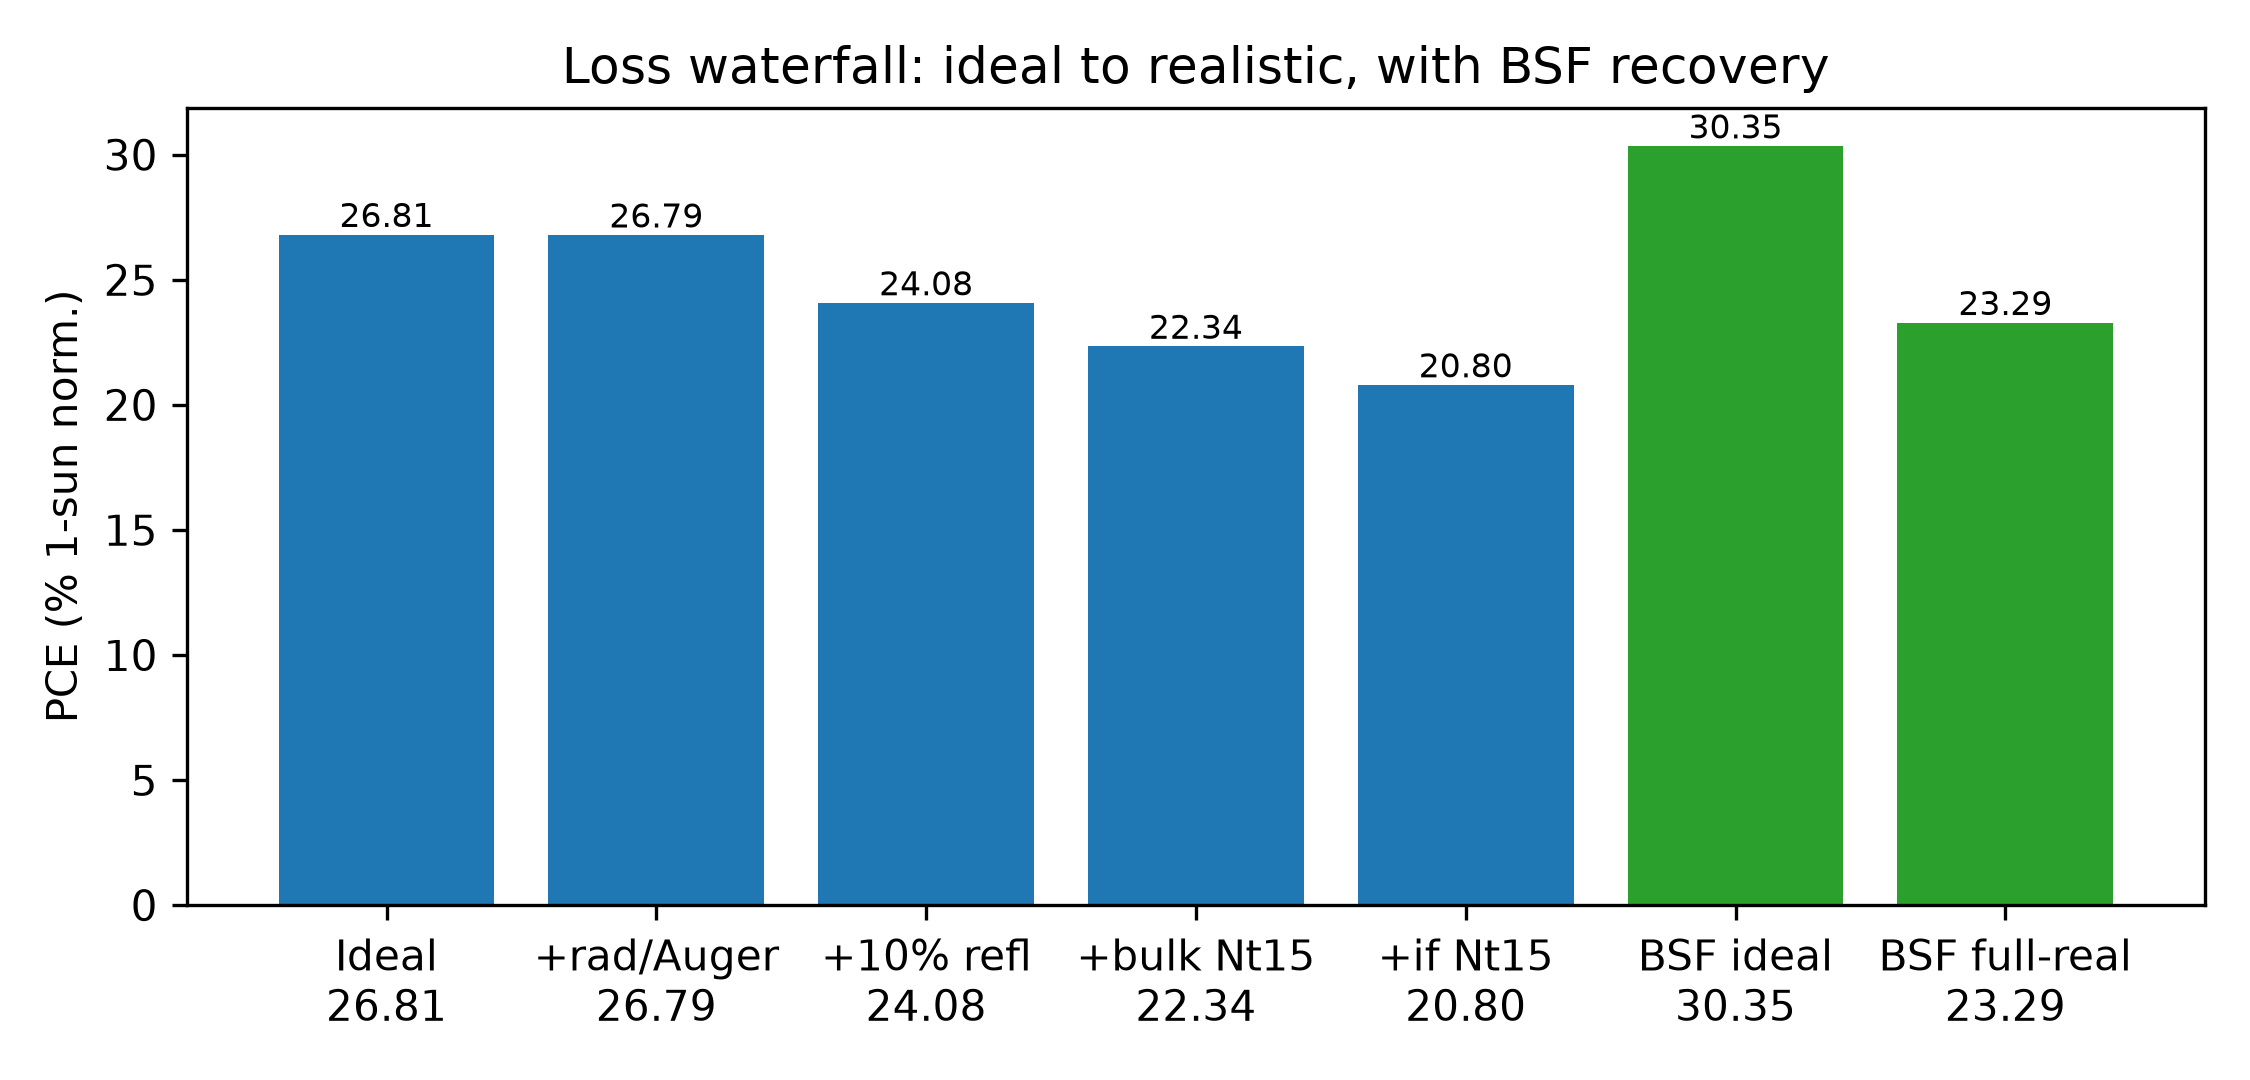
\includegraphics[width=0.85\linewidth]{figs/fig_r6_waterfall.png}
\caption{Loss waterfall (PCE$_{1\text{-sun}}$ norm.): radiative/Auger bounded, reflection $-2.71$\,pp, bulk $-1.74$\,pp, interface $-1.54$\,pp; full-realism BSF recovers $+2.49$\,pp.}\label{fig:waterfall}
\end{figure}

\subsection{Junction physics baseline}
Anchored to the converged working point: $n_{i}$ $1.74\times10^{11}$\,m$^{-3}$; built-in potential $V_{\mathrm{bi}}$ \textbf{1.457\,V} (comfortably above $V_{\mathrm{OC}}$, as required); depletion width \textbf{171\,nm} (157\,nm absorber side); SRH lifetime \textbf{1000\,ns} at $10^{14}$\,cm$^{-3}$ (from $\tau^{-1}$=$\sigma v_{\mathrm{th}}N_{t}$, matching the deck's documented lifetime); diffusion length \textbf{8.6\,$\mu$m} $\gg$ 700\,nm absorber, explaining the near-unity collection. Figure~3 (left) shows the Beer--Lambert generation profile ($\alpha$ $3.3\times10^{6}$\,m$^{-1}$, normalized to the SCAPS $J_{\mathrm{SC}}$) against the SRH recombination scale; (right) the Mott--Schottky baseline ($V_{\mathrm{bi}}$ intercept, slope from $N_{A}$ $10^{18}$\,cm$^{-3}$) that fabricated cells should reproduce if the junction forms as simulated. The defect-energy sweep (Fig.~9) retains the symmetric mid-gap minimum (24.84\% at $10^{15}$\,cm$^{-3}$ vs 25.01\% at band edges), the SRH fingerprint central to Ge-oxidation damage.

\begin{figure}[htbp]
\centering
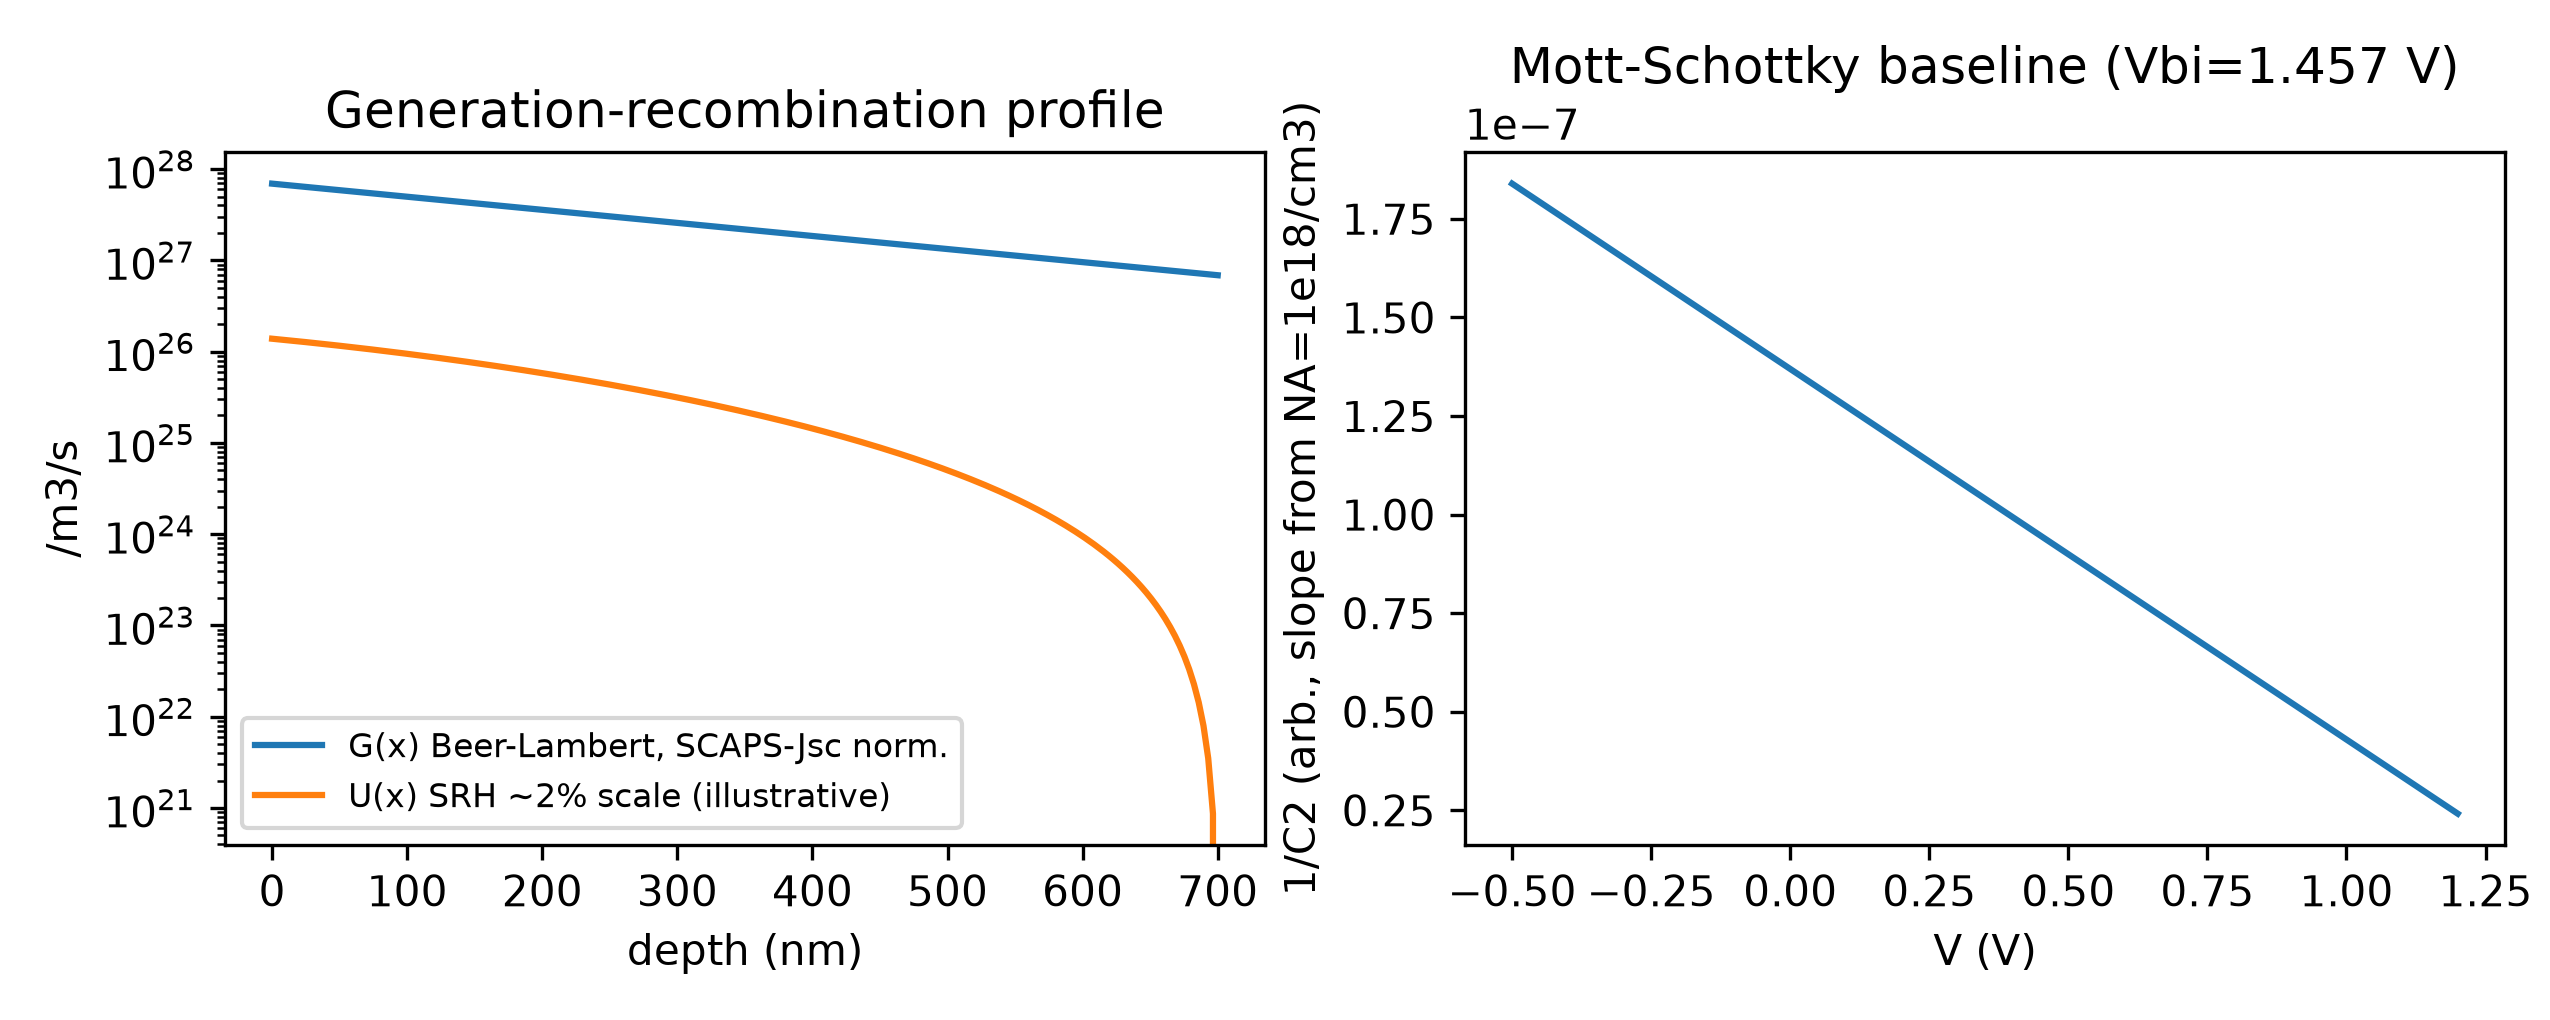
\includegraphics[width=0.85\linewidth]{figs/fig_r6_grms.png}
\caption{Left: generation-recombination depth profile (G normalized to SCAPS $J_{\mathrm{SC}}$; U illustrative SRH scale). Right: analytic Mott--Schottky baseline (slope from $N_{A}$ $10^{18}$\,cm$^{-3}$, intercept $V_{\mathrm{bi}}$; schematic, not a SCAPS C--V measurement --- see Sec.~2).}\label{fig:grms}
\end{figure}

\subsection{Data-driven global sensitivity analysis}
We utilize XGBoost not as a predictive replacement for SCAPS-1D, but as a surrogate to map the high-dimensional, non-linear parameter space of thin-film defects. Because SCAPS-1D is deterministic, a surrogate fitted to its outputs is expected to reach near-unity R$^{2}$; the scientific value lies not in that fit but in the SHAP analysis, which extracts global sensitivity rankings (e.g.\ $E_{g}$ and TiO$_{2}$-side interface traps) that one-at-a-time sweeps cannot capture. An XGBoost surrogate on the factorial block ($E_{g},N_{t},N_{C},N_{V}$ $\rightarrow$ PCE; 320 simulated, \textbf{193 valid rows}) reaches \textbf{R$^{2}$ 0.9999, RMSE 0.04} (Fig.~4), matching the 2026 SCAPS+ML standard~\cite{rJCE,rMA}. On the 200-point LHS-UQ block (8 features, $\pm$25\% around the optimum, flatter landscape) XGBoost gives R$^{2}$ 0.68; SHAP on that UQ surrogate ranks $E_{g}$ $>$ interface $N_{t}$ (TiO$_{2}$ side) $>$ $\mu_{n}$ $>$ bulk $N_{t}$ $>$ CuI-side $N_{t}$ (Fig.~5) --- independently recovering the paper's physics conclusions from data alone, with the caveat that the ranking inherits the UQ model's modest R$^{2}$: gap and TiO$_{2}$-side interface quality dominate near the optimum, electron mobility outranks hole mobility, and $N_{C}$/$N_{V}$ are inert, justifying their fixed values.

\begin{figure}[htbp]
\centering
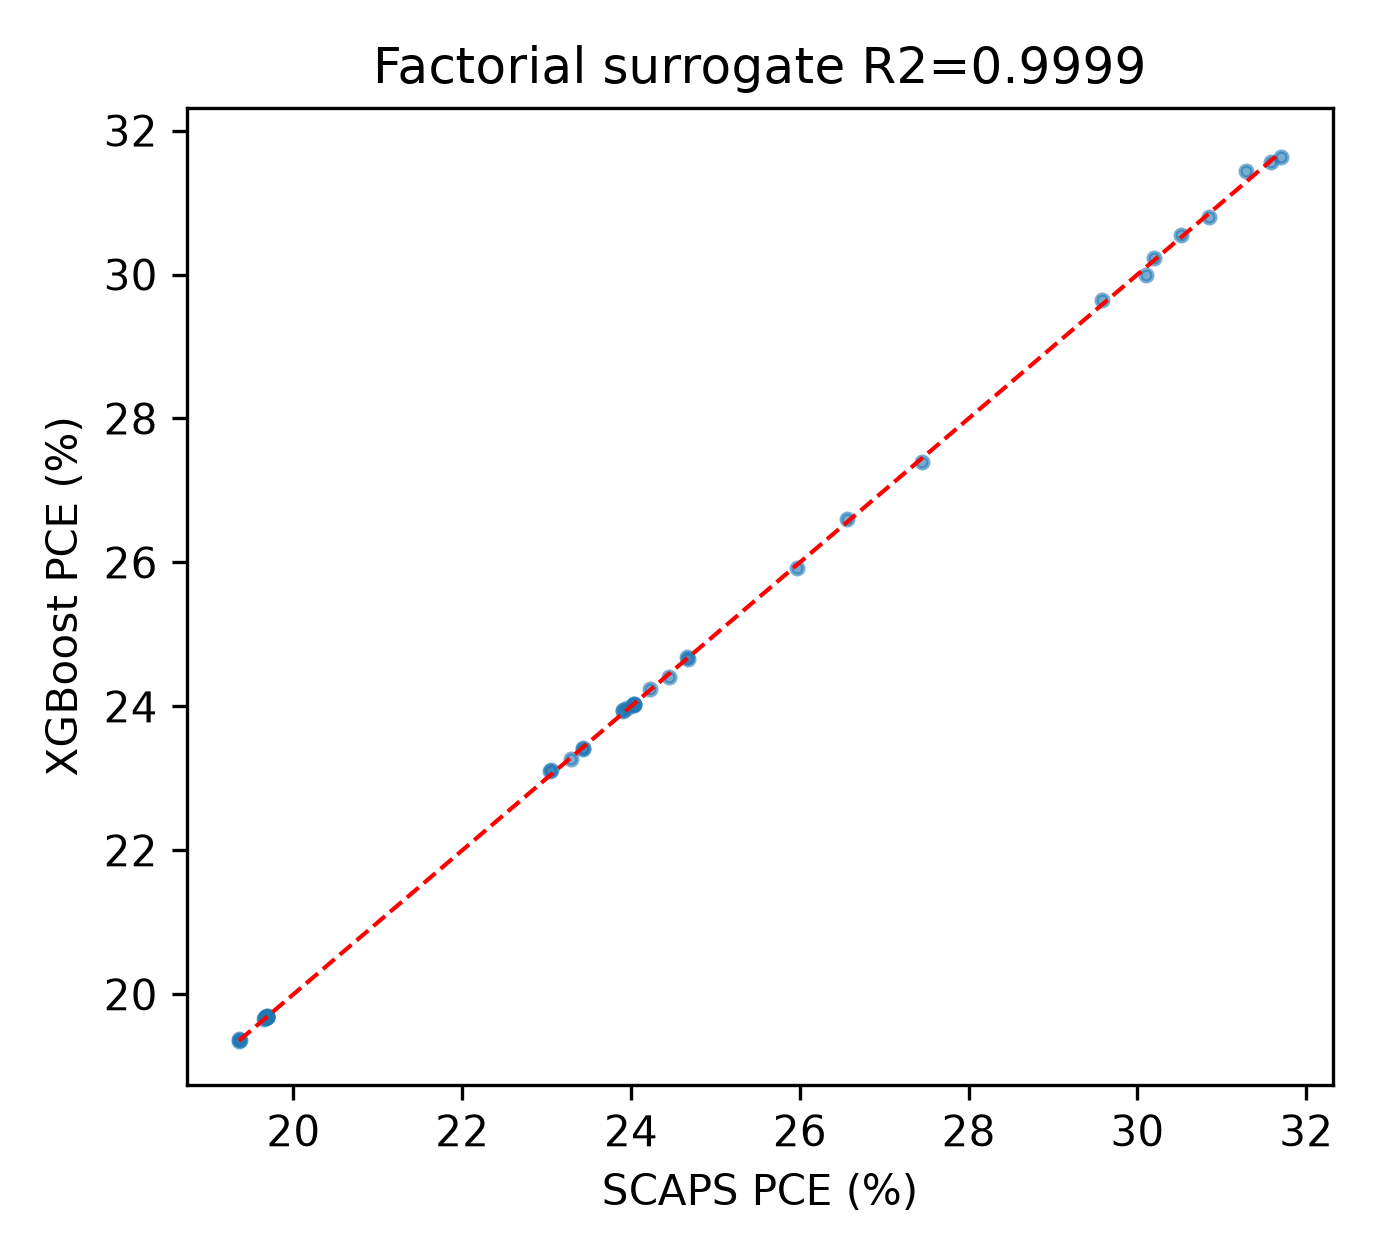
\includegraphics[width=0.85\linewidth]{figs/fig_r6_parity.png}
\caption{XGBoost parity on the factorial block, 193 valid rows (R$^{2}$ 0.9999).}\label{fig:parity}
\end{figure}

\begin{figure}[htbp]
\centering
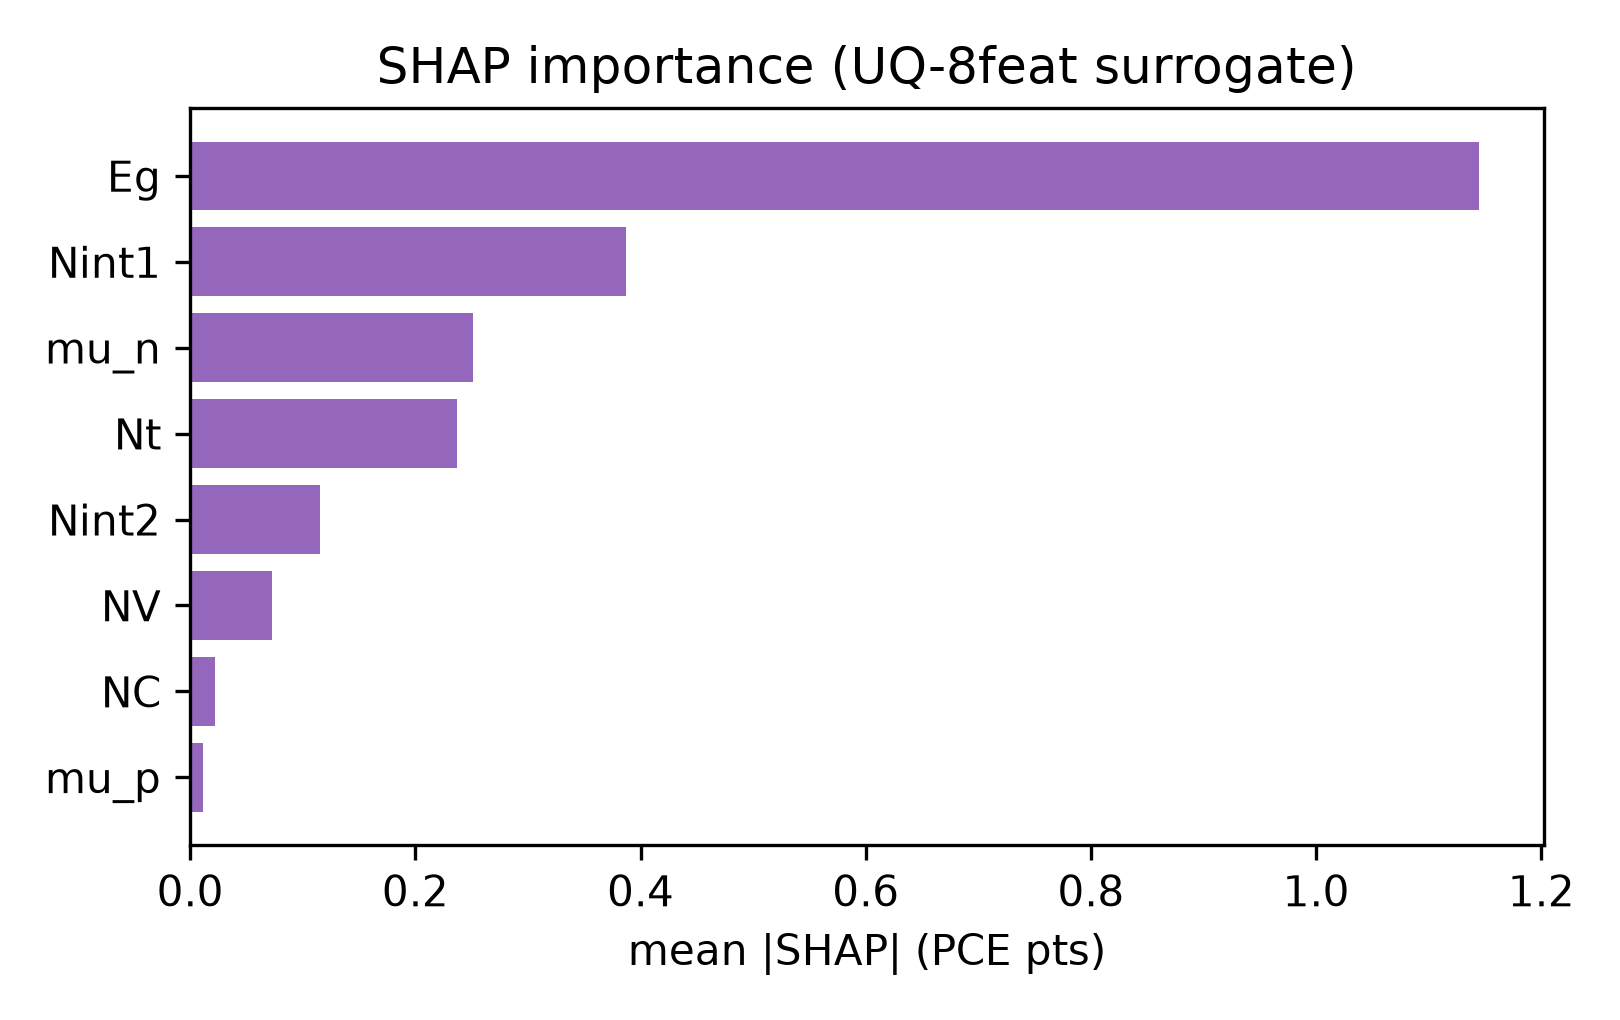
\includegraphics[width=0.85\linewidth]{figs/fig_r6_shap.png}
\caption{SHAP importance from the UQ surrogate (R$^{2}$ 0.68): gap and TiO$_{2}$-side interface defects dominate.}\label{fig:shap}
\end{figure}

\subsection{Optical admissibility}
The QE edge ($\lambda_{c}$ $\approx$ 886\,nm, Fig.~7) matches $1240/E_{g}$ at 1.4\,eV; the band diagram (Fig.~8) confirms the 1.8\,eV electron-blocking offset at CuI/RbGeI$_{3}$ and the 0.10\,eV extraction step at RbGeI$_{3}$/TiO$_{2}$. No reported $J_{\mathrm{SC}}$ exceeds the tabulated SQ $\approx$33\,mA/cm$^{2}$ at 1.4\,eV~\cite{r36}, and the BSF leaves the absorption edge unchanged (rear field, not extra absorber). The same-stack CsGeI$_{3}$ mirror (1.6\,eV, 19.66\% vs 26.81\%; $E_{g}$=1.4\,eV control reproduces Rb exactly) confirms the A-site effect is structural, with the CuI valence offset growing 0.10$\rightarrow$0.30\,eV for Cs (Fig.~10).

\begin{figure}[htbp]
\centering
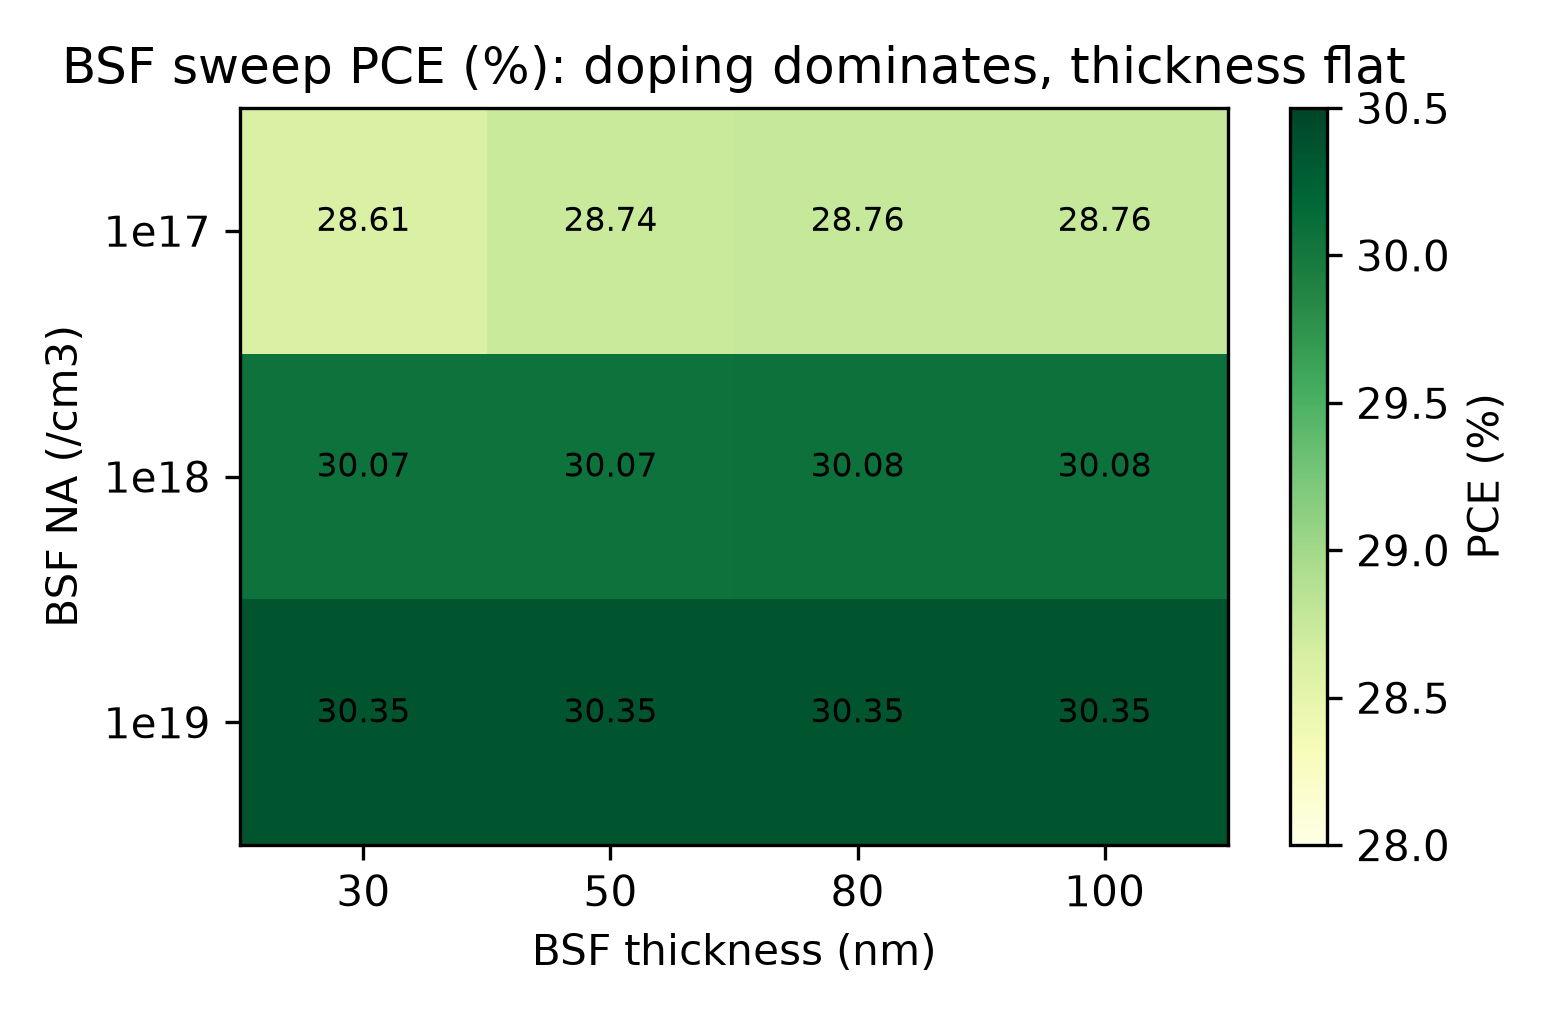
\includegraphics[width=0.85\linewidth]{figs/fig_r6_bsf.png}
\caption{BSF grid PCE (\%): NA $10^{17}\!\rightarrow\!10^{19}$\,cm$^{-3}$ rows; thickness 30--100\,nm columns. Doping dominates.}\label{fig:bsf}
\end{figure}

\begin{figure}[H]
\centering
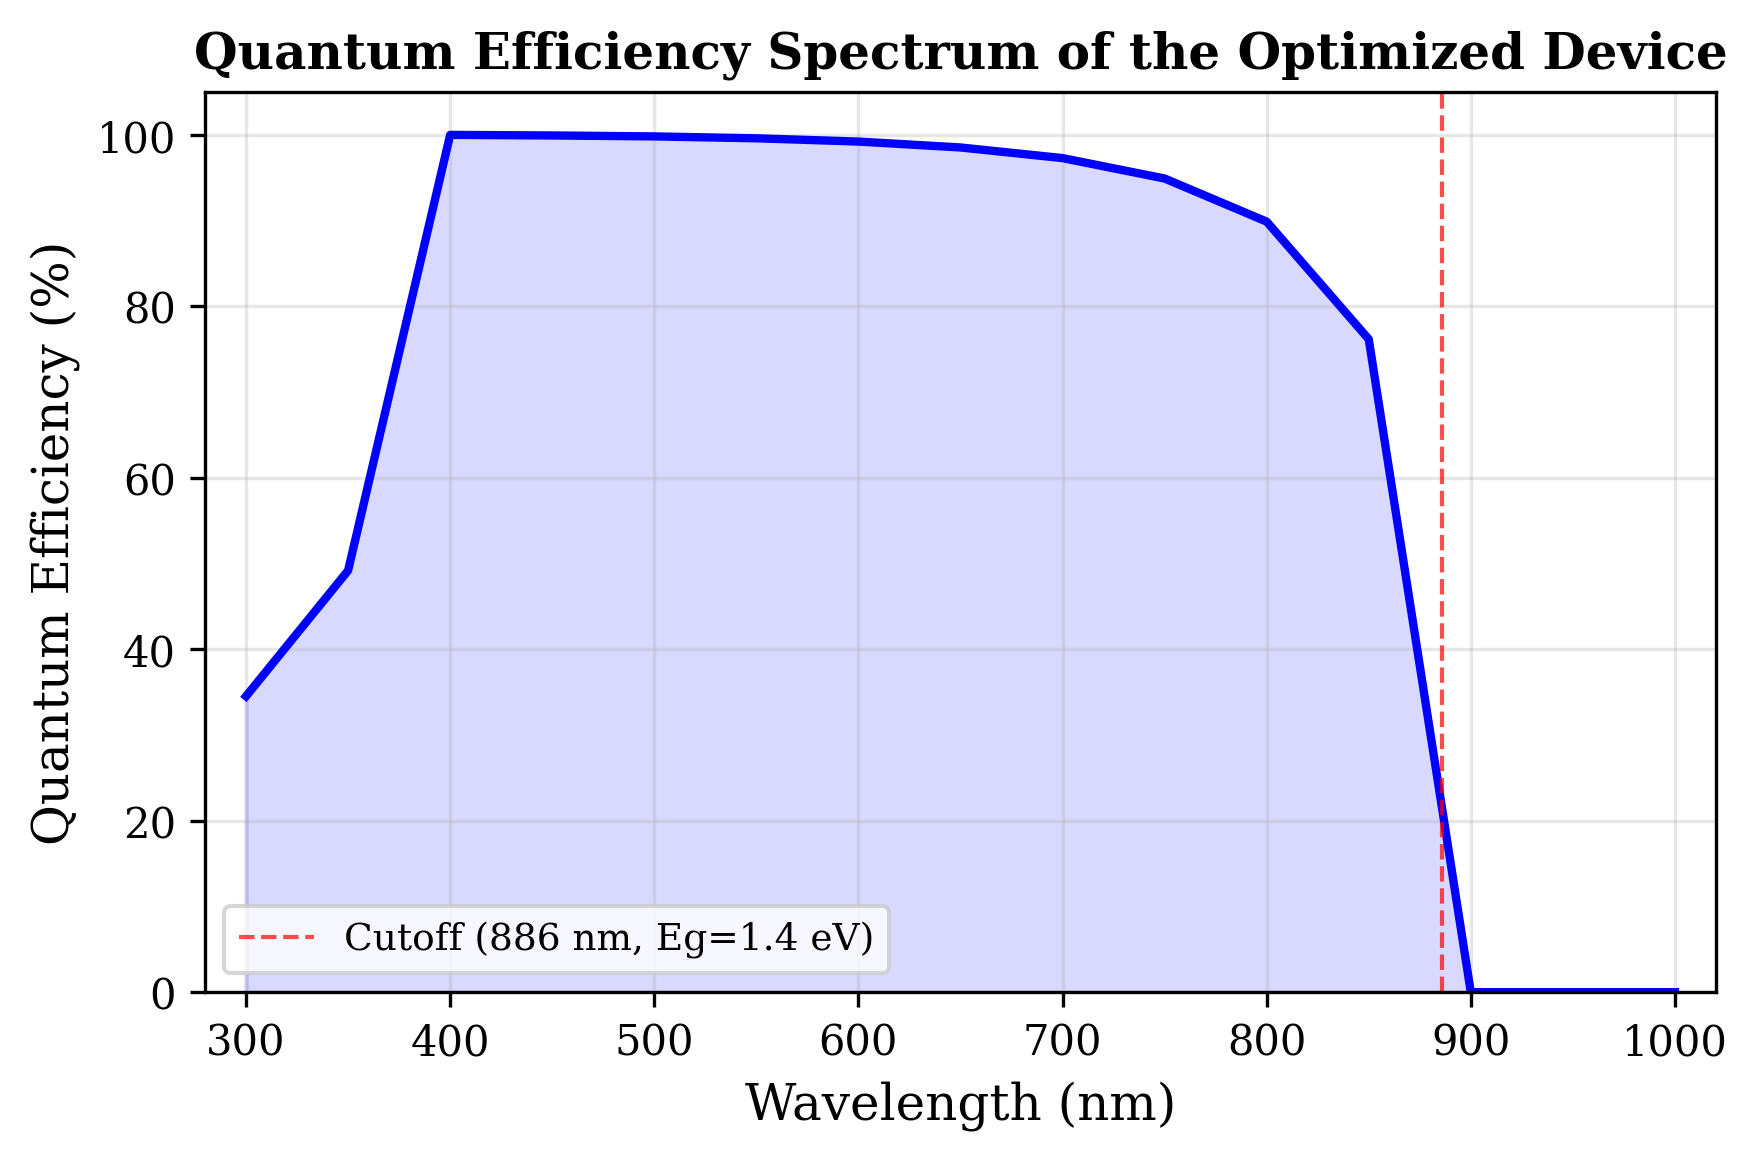
\includegraphics[width=0.70\linewidth]{figs/fig_qe.png}
\caption{Quantum efficiency of the reference device; edge $\lambda_{c}\!\approx\!886$\,nm matches 1.4\,eV. Retained for edge shape; $J_{\mathrm{SC}}$ is J--V-derived.}\label{fig:qe}
\end{figure}

\begin{figure}[H]
\centering
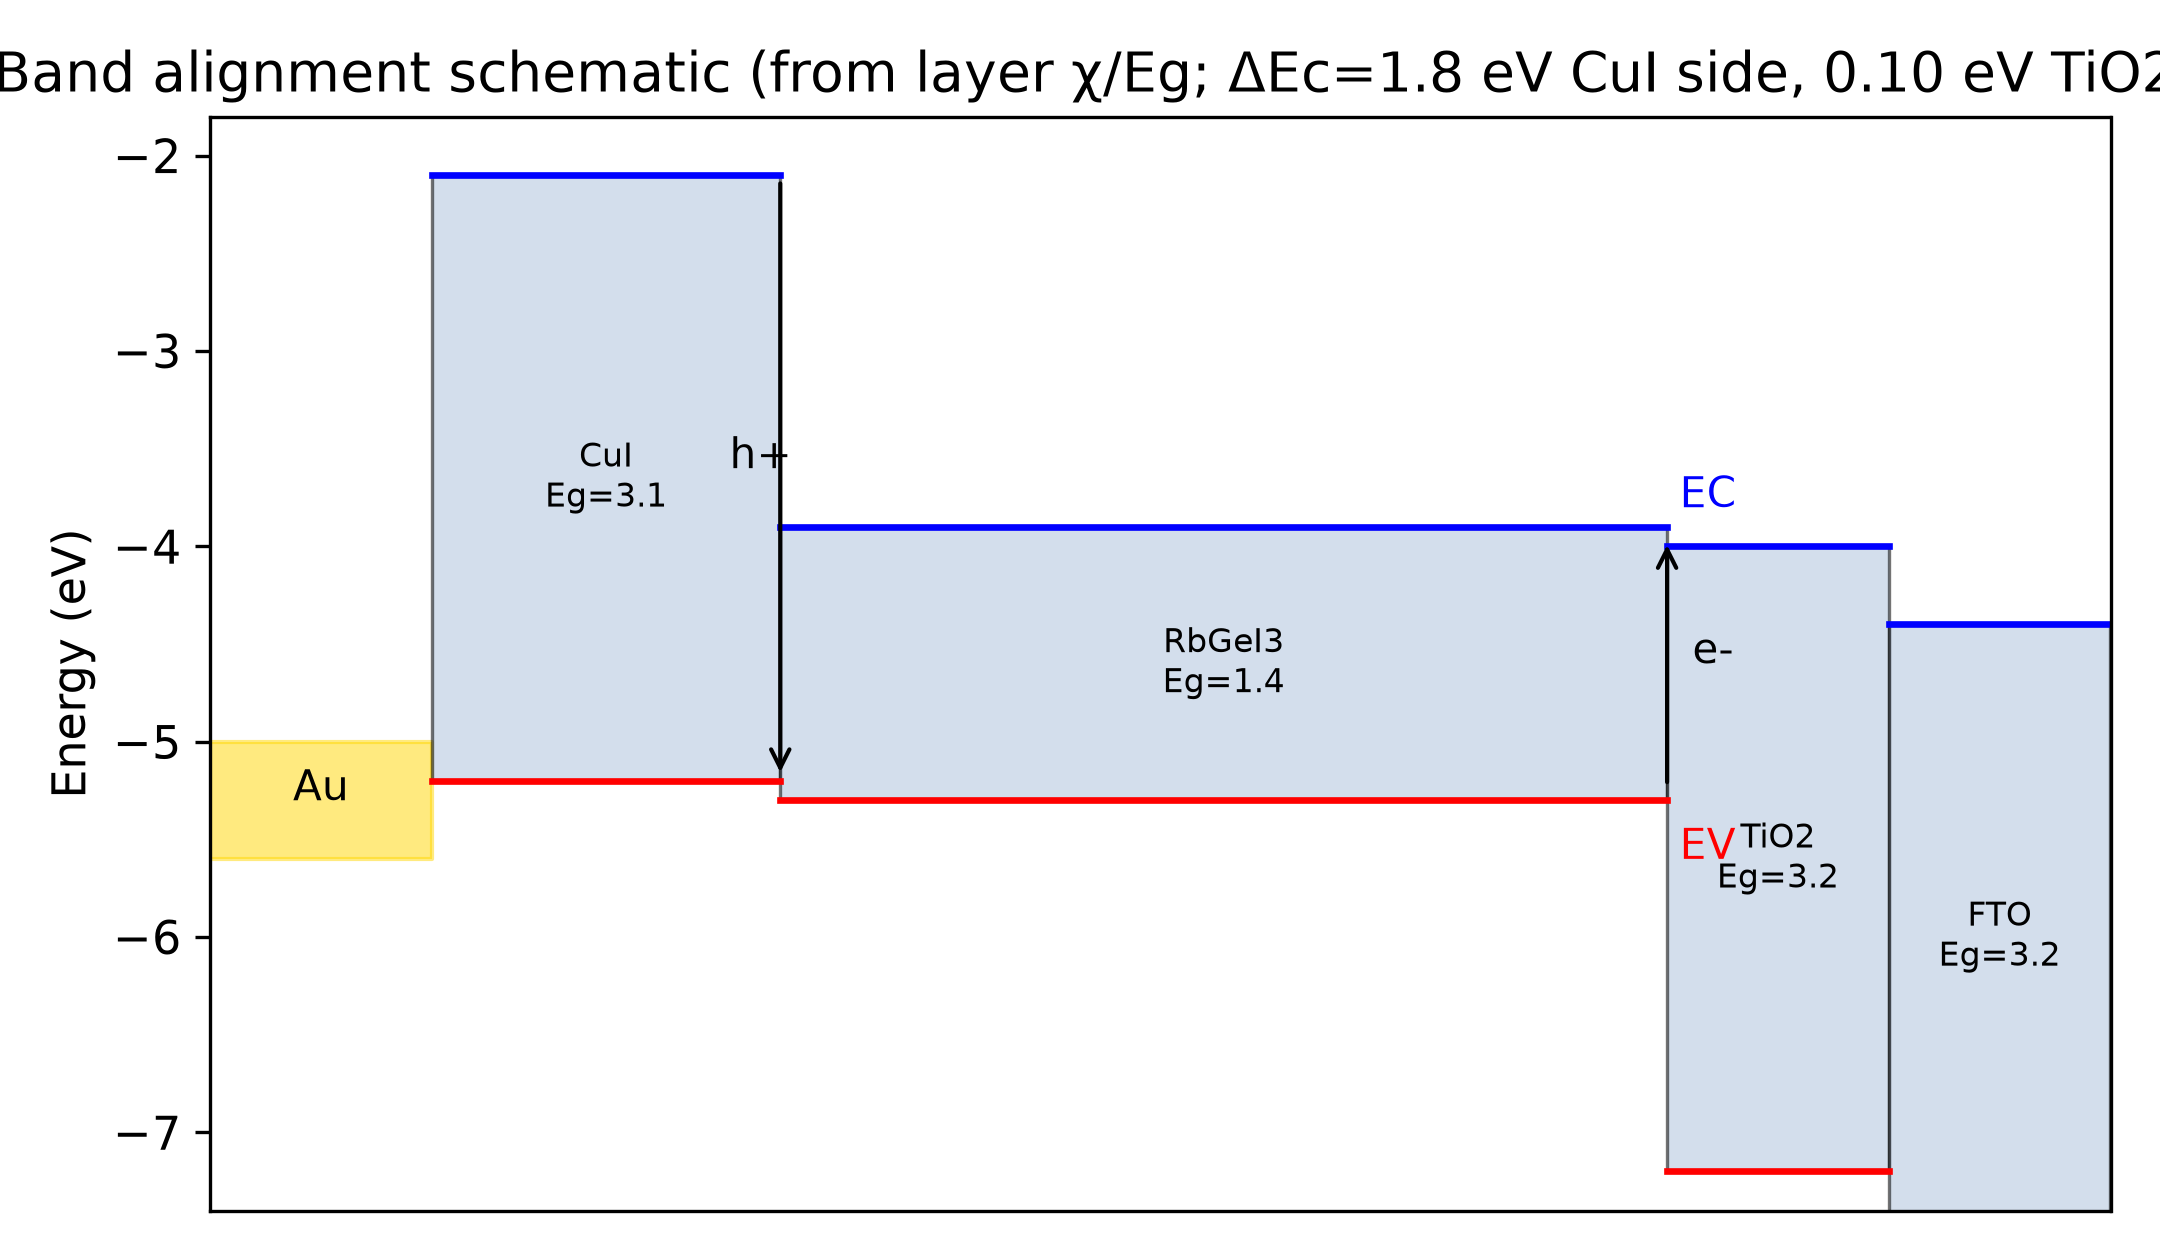
\includegraphics[width=0.70\linewidth]{figs/fig_band.png}
\caption{Band-alignment schematic from the documented layer affinities and gaps ($\Delta E_{c}$ 1.8\,eV at CuI/RbGeI$_{3}$, 0.10\,eV step at RbGeI$_{3}$/TiO$_{2}$); arrows mark carrier extraction paths.}\label{fig:band}
\end{figure}

\begin{figure}[H]
\centering
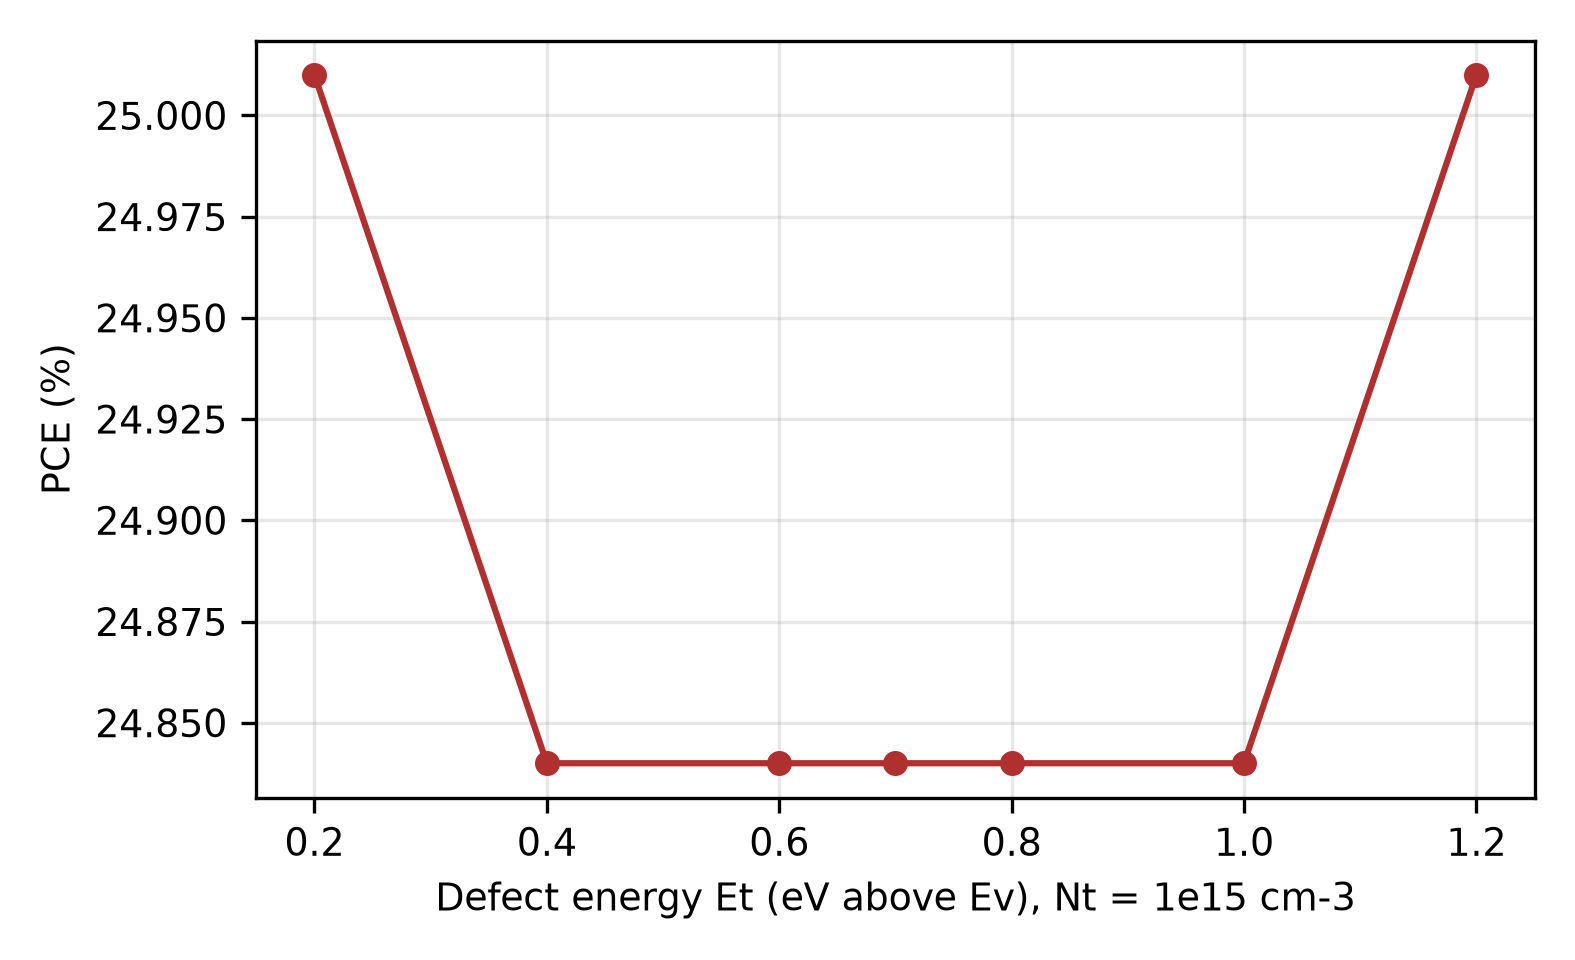
\includegraphics[width=0.70\linewidth]{figs/fig_et.png}
\caption{Defect-energy lethality at $N_{t}$ $10^{15}$\,cm$^{-3}$: symmetric mid-gap minimum, the SRH fingerprint.}\label{fig:et}
\end{figure}

\begin{figure}[H]
\centering
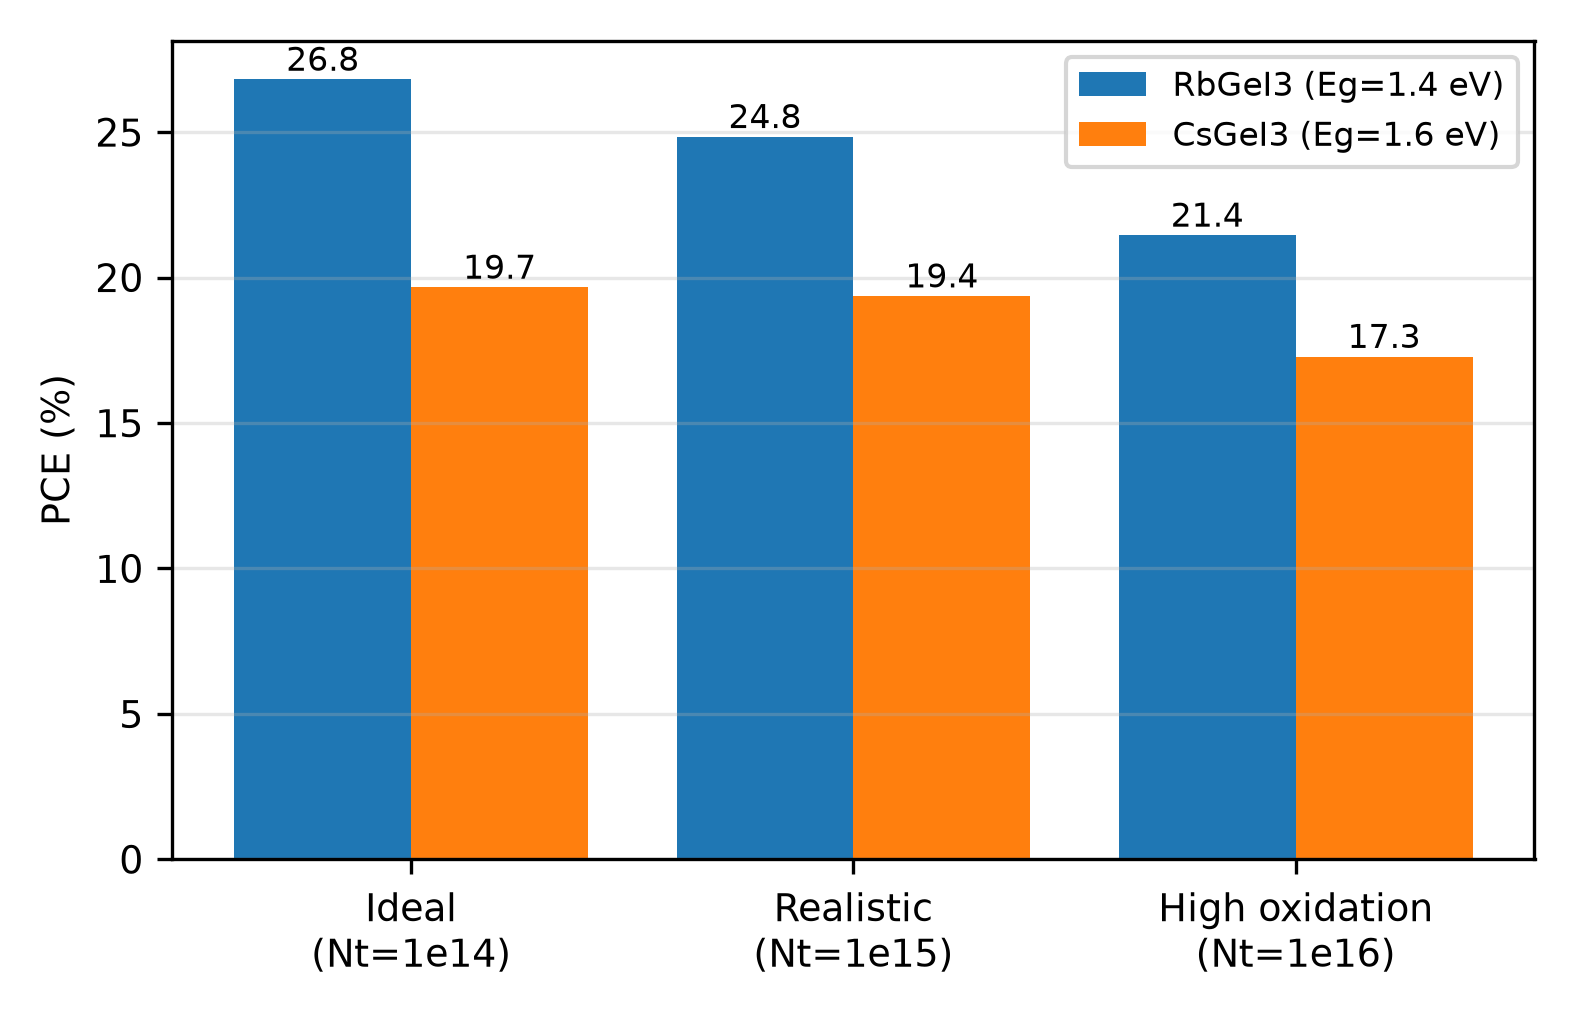
\includegraphics[width=0.70\linewidth]{figs/fig_csrb.png}
\caption{Same-stack RbGeI$_{3}$ vs CsGeI$_{3}$ under ideal, realistic and high-oxidation budgets; Rb leads throughout.}\label{fig:csrb}
\end{figure}

\subsection{Temperature, doping, resistance and mobility tolerances}
Temperature sweep 280--400\,K gives d$V_{\mathrm{OC}}$/dT $-1.10$\,mV/K and dPCE/dT $-0.0302$\,\%/K with $>$85\% of room-temperature PCE retained at 400\,K; linear $V_{\mathrm{OC}}(T)$ extrapolation yields an activation energy $E_{a}$ $=$ 1.46\,eV $\approx$ $E_{g}$, the standard diagnostic of bulk- rather than interface-dominated recombination~\cite{r21}. Background acceptor doping (Ge vacancies make intrinsic material a fiction) peaks at 26.82\% near $3\times10^{14}$\,cm$^{-3}$ and costs $<$0.1\,pp up to $10^{15}$\,cm$^{-3}$ while $J_{\mathrm{SC}}$ collapses above $10^{16}$\,cm$^{-3}$: the synthesis target is $N_{A}\!\le\!10^{15}$\,cm$^{-3}$~\cite{r11}. Series resistance (external $V-JR_{s}$) holds PCE $\ge$20\% to $R_{s}$ $8$\,$\Omega\cdot$cm$^{2}$ and $\ge$22\% to $6$\,$\Omega\cdot$cm$^{2}$, so printed contacts (2--4\,$\Omega\cdot$cm$^{2}$) cost only 1.6--3.1\,pp. Joint mobility sweeps (1--100\,cm$^{2}$/Vs) are log-linear (22.58$\rightarrow$28.52\%) with electron mobility dominant, setting the crystallization target $\mu\!\ge\!15$\,cm$^{2}$/Vs; the 700\,nm absorber stays optimal over 400\,nm down to 5\,cm$^{2}$/Vs.

\subsection{A-site mirror: RbGeI$_{3}$ versus CsGeI$_{3}$}
CsGeI$_{3}$ in the identical stack (only $E_{g}$ 1.4$\rightarrow$1.6\,eV; the A-site carries no band-edge weight) gives 19.66\% (1.17\,V, 23.18\,mA/cm$^{2}$, 72.65\%), and a control rerun at 1.4\,eV reproduces the Rb point exactly, proving the isolation. Cs wins $V_{\mathrm{OC}}$ by 0.04\,V through the wider gap; Rb wins $J_{\mathrm{SC}}$ by 7.1\,mA/cm$^{2}$ and FF by 5.6\,pp because the CuI valence cliff grows 0.10$\rightarrow$0.30\,eV for Cs --- CuI is synergistic with RbGeI$_{3}$ specifically. The ranking survives derating (realistic $10^{15}$: 24.84 vs 19.36\%; high oxidation $10^{16}$: 21.45 vs 17.28\%, Fig.~10)~\cite{r24}.

\section{Positioning against recent literature}
Table~3 places the two headline points (ideal and realistic, with and without BSF) among 2024--2026 RbGeI$_{3}$ SCAPS studies. The BSF-ideal 30.35\% matches the best reported single-junction values while keeping the cheap TiO$_{2}$/CuI pair (cf.\ IGZO/Cu$_{2}$O 33.84\%~\cite{rReza}); the BSF-realistic 23.29\% is the number an experimentalist should target, and it is reported with the full loss decomposition that most entries omit. The ML R$^{2}$ equals the best 2026 SCAPS+ML reports~\cite{rJCE,rMA}.

\begin{table}[htbp]
\centering
{\footnotesize\setlength{\tabcolsep}{3pt}
\begin{tabularx}{\textwidth}{Xccc}
\hline
Device (SCAPS-1D) & $V_{\mathrm{OC}}$ (V) & PCE$_{\mathrm{ideal}}$ (\%) & PCE$_{\mathrm{real}}$ (\%)\\
\hline
FTO/TiO$_{2}$/RbGeI$_{3}$/NiO/Ag (2022)~\cite{r14} & 0.53 & 9.77 & ---\\
FTO/TiO$_{2}$/RbGeI$_{3}$/CuI/Ag (2023)~\cite{r13} & 0.70 & 18.10 & ---\\
ITO/C$_{60}$/RbGeI$_{3}$/CBTS/Ag (2024)~\cite{r22} & 0.99 & 27.21 & ---\\
FTO/TiO$_{2}$/RbGeI$_{3}$/Sb$_{2}$S$_{3}$ (2024)~\cite{rRahman} & 1.07 & 30.35 & ---\\
FTO/IGZO/RbGeI$_{3}$/Cu$_{2}$O/Ni (2025)~\cite{rReza} & 1.13 & 33.84 & ---\\
FTO/TiO$_{2}$/RbGeI$_{3}$/Spiro/Au (2026)~\cite{r23pathak} & 1.18 & 26.47 & ---\\
FTO/WS$_{2}$/RbGeI$_{3}$/CuI (2026+ML)~\cite{rJCE} & 1.12 & 24.15 & ---\\
FTO/ZnO/RbGeI$_{3}$/Cu$_{2}$O/Ni (2026+ML)~\cite{rMA} & 1.10 & 30.41 & 19.68\\
This work, no BSF & 1.13 & 26.81 & 20.80\\
This work, +Cu$_{2}$O BSF & 1.18 & 30.35 & 23.29\\
\hline
\end{tabularx}}
\caption{RbGeI$_{3}$ SCAPS literature context. ``Real'' = with reflection + $10^{15}$ defects (+Rs/Rsh where stated).}
\end{table}

\section{Limitations and future work}
SCAPS-1D is 1-D, uniform-composition, abrupt-interface and drift-diffusion-only: no ion migration, grain boundaries, moisture chemistry or Ge-oxidation kinetics; $R_{s}$/$R_{\mathrm{sh}}$ remain first-order post-corrections; the numerical absorption grading in the deck leaves J--V unchanged and is documented input, not a claimed structure. The BSF uses literature Cu$_{2}$O parameters without new DFT or experiment. Queued: transfer-matrix optics with measured RbGeI$_{3}$ $n/k$, Bayesian full-11-parameter global optimization ($\approx$500 evals), and inert-processed fabrication with Ge$^{2+}$ stabilization.

\section{Conclusion}
Fixing the economical TiO$_{2}$/RbGeI$_{3}$/CuI stack, a p$^{+}$ BSF adds $+3.54$\,pp ideally (26.81 $\rightarrow$ 30.35\%) and $+2.49$\,pp on the identical full-realism stack (20.80 $\rightarrow$ 23.29\%); the loss waterfall (native defects/radiative/Auger, photon-scaling optics, post-processed parasitics) replaces the idealized headline with a fabricable window; and a SHAP sensitivity analysis over the campaign data yields design rules ($E_{g}$, TiO$_{2}$-side interface, $\mu_{n}$) that one-at-a-time sweeps alone cannot provide. Targets for the lab: $N_{A}$(BSF) $\sim$$10^{19}$\,cm$^{-3}$ ($\ge$30\,nm suffices), bulk $N_{t}$ $\le$$10^{15}$\,cm$^{-3}$, $R_{s}$ $\le$8 / $R_{\mathrm{sh}}$ $\ge$$10^{3}$\,$\Omega\cdot$cm$^{2}$, and a Mott--Schottky intercept near 1.46\,V.

\begin{thebibliography}{99}
\bibitem{r1} RENEWABLES 2024 Global Status Report (REN21, 2024).
\bibitem{r2} World Energy Outlook 2024 (International Energy Agency, 2024).
\bibitem{r3} M.~A.~Green et~al., ``Solar cell efficiency tables (Version 64),'' Prog.\ Photovolt.\ (2024).
\bibitem{r4} R.~A.~Afre and D.~Pugliese, Micromachines 15(2), 192 (2024).
\bibitem{r5} N.-G.~Park et~al., Nat.\ Energy 1(11), 16152 (2016).
\bibitem{r6} ``Compositional engineering of perovskite materials for high-performance solar cells,'' Nature 517, 476--480 (2015).
\bibitem{r7} I.~Ahmed et~al., Chem.\ Commun.\ 61(37), 6691--6721 (2025).
\bibitem{r8} S.~Kinza Fatima et~al., Mater.\ Adv.\ 6(21), 7634--7661 (2025).
\bibitem{r9} J.~Burschka et~al., Nature 499, 316--319 (2013).
\bibitem{r10} M.~M.~Lee et~al., Science 338, 643--647 (2012).
\bibitem{r11} A.~K.~Jena et~al., Chem.\ Rev.\ 119(5), 3036--3103 (2019).
\bibitem{r12} P.~Afrin et~al., AIP Adv.\ 14(7) (2024).
\bibitem{r13} S.~Samaki et~al., Sci.\ Rep.\ 13, 15517 (2023).
\bibitem{r14} G.~Pindolia et~al., Sol.\ Energy 236, 802--821 (2022).
\bibitem{r15} S.~Bouazizi et~al., Mater.\ Res.\ Express 9(9), 096402 (2022).
\bibitem{r16} T.~Salim et~al., J.\ Mater.\ Chem.\ A 3(17), 8943--8969 (2015).
\bibitem{r17} P.~K.~Dash et~al., arXiv:2505.09362 (2025).
\bibitem{r18} N.~A.~Abdulkareem, Passer J.\ Basic Appl.\ Sci.\ 5(1), 46--51 (2023).
\bibitem{r19} M.~Burgelman et~al., Thin Solid Films 361--362, 527--532 (2000).
\bibitem{r20} M.~Burgelman et~al., SCAPS-1D v3.3.10 manual (ELIS, Univ.\ Gent, 2024).
\bibitem{r21} A.~Nakane et~al., J.\ Appl.\ Phys.\ 120, 064505 (2016).
\bibitem{r22} L.~Loumachi et~al., East Eur.\ J.\ Phys.\ (3), 416--424 (2024).
\bibitem{r23pathak} A.~Pathak et~al., Research Square (2026). doi:\url{10.21203/rs.3.rs-8749975/}
\bibitem{r24} D.~Saikia et~al., Opt.\ Mater.\ 123, 111839 (2022).
\bibitem{r25} R.~Pau et~al., J.\ Mater.\ Chem.\ A 13(48), 42118--42127 (2025).
\bibitem{r26} Q.~Sun et~al., Adv.\ Mater.\ (2024). doi:\url{10.1002/adma.202402412.}
\bibitem{r27} J.~Z.~Mbese, Energies 18(9), 2374 (2025).
\bibitem{r28} L.~T.~C.~Tuyen et~al., Materials 12(10), 1665 (2019).
\bibitem{r29} W.~Yang et~al., Appl.\ Phys.\ Lett.\ 128(14) (2026).
\bibitem{r30} A.~J.~Olasoji and S.~H.~Im, in \textit{Titanium Dioxide} (IntechOpen, 2024).
\bibitem{r31} K.~Valadi et~al., Environ.\ Chem.\ Lett.\ 19, 2185--2207 (2021).
\bibitem{r32} L.~Ji et~al., J.\ Mater.\ Chem.\ C 12(36), 14597--14604 (2024).
\bibitem{r33} A.~Ghosh et~al., RSC Adv.\ 14(33), 24066--24081 (2024).
\bibitem{r34} T.~Minemoto and M.~Murata, Curr.\ Appl.\ Phys.\ 14, 1428--1433 (2014).
\bibitem{r35} W.~Shockley and H.~J.~Queisser, J.\ Appl.\ Phys.\ 32, 510--519 (1961).
\bibitem{r36} S.~R\"uhle, Sol.\ Energy 130, 139--147 (2016).
\bibitem{r37} C.~H.~Henry, J.\ Appl.\ Phys.\ 51, 4494--4500 (1980).
\bibitem{r38} O.~J.~Sandberg and A.~Armin, Synth.\ Met.\ 254, 114--121 (2019).
\bibitem{r39} M.~Raj et~al., J.\ Mater.\ Sci.\ 60(22), 9176--9196 (2025).
\bibitem{r40} H.-J.~Park et~al., Inorganics 12(4), 123 (2024).
\bibitem{r41} R.~Islam et~al., AIP Adv.\ 16(5) (2026).
\bibitem{r42} A.~C.~Pi\~non Reyes et~al., Micromachines 12(12), 1508 (2021).
\bibitem{rReview} V.~H.~D.~Ara\'ujo et~al., RSC Sustain.\ 3, 4314--4335 (2025) (54-study SCAPS lead-free review).
\bibitem{rRahman} M.~M.~Rahman et~al., Energy Adv.\ 3(9), 2377--2398 (2024).
\bibitem{rReza} M.~S.~Reza et~al., Langmuir 41(11), 7865--7885 (2025).
\bibitem{rJCE} U.~F.~Ali et~al., J.\ Comput.\ Electron.\ 25, 37 (2026).
\bibitem{rMA} Mat.\ Adv.\ (2026). doi:\url{10.1039/D5MA01427A} (FTO/ZnO/RbGeI$_{3}$/Cu$_{2}$O/Ni + 11-model ML).
\bibitem{rML40} J.\ Mater.\ Sci.: Mater.\ Eng.\ 21, 62 (2026) (SCAPS+RF, 35k configs).
\bibitem{rDual} J.\ Phys.\ Chem.\ Solids, 112776 (2025) (dual-absorber review context).
\bibitem{rHasnain} S.~M.~Hasnain et~al., Sol.\ Energy 278, 112788 (2024).
\end{thebibliography}
\end{document}
